\Kilian{}

\Moritz{
	
\begin{frame}{Zu ÜB 3}
	
	Allgemein:
	\begin{itemize}
		\item \enquote{Geben Sie an} $\Rightarrow$ Nur Lösung reicht!
		\item Ich bewerte auch nur die endgültige Lösung
		\item Begründungen/Erklärungen ignoriere ich (größtenteils)
	\end{itemize}

\end{frame}
		
\begin{frame}{Zu ÜB 3}

	Aufgabe 3.5 (d):\\[.3em]

	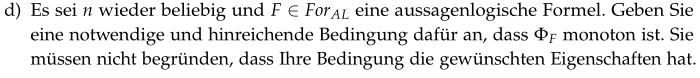
\includegraphics[width=\textwidth]{../topics/orga/WS2021_Aufg_3_5_d}

	\begin{itemize}
		\item Korrekturanweisung von Worschanese: Definition der Monotonie (oder ähnliche Formulierungen) geben keine Punkte
		\item Ziel der Aufgabe: Zusammenhang zwischen Formel $F$ und Monotonie der Funktion $\Phi_F$ finden
		\pause
		\item Lösung: \begin{itemize}
			\item Idee: Negation $\bnot$ und Implikation $\bimp$ können selbst bei $x \preceq y$ zu $\Phi_F(x) \npreceq \Phi_F(y)$ führen
			\item Aber Achtung: In $F$ selbst darf $\bnot$ und $\bimp$ vorkommen, solange es eine zu $F$ logisch äquivalente Formel $G$ gibt, die kein $\bnot$ oder $\bimp$ enthält
			% \item z.B. $n=1$, $F = \bnot\bnot P_0$, $G = P_0$ $\Rightarrow$ $\Phi_F$ ist monoton
			\item Außerdem gilt: Wenn $F$ eine Tautologie oder unerfüllbar ist, so ist $\Phi_F$ immer monoton
		\end{itemize}
	\end{itemize}


\end{frame}

}
